\documentclass[11pt]{article}
\usepackage[margin=1in]{geometry}
\usepackage{amsmath,amssymb}
\usepackage{graphicx}
\usepackage{booktabs}
\usepackage[colorlinks=true,linkcolor=black,citecolor=black,urlcolor=black]{hyperref}
\usepackage{times}

\title{\textbf{Hidden Twins in the Training Set: Subject-Level Data Leakage Inflates Machine-Learning Performance in Voice-Based Parkinson's Disease Assessment, and a Design-Effect Identity Tracks the Size of the Bias}}

\author{Mustafojon Tursunbadalov$^{*1}$, Muhammadjon Tursunbadalov$^{*1}$, and Bekir Karlik$^{2}$}
\date{}

\begin{document}
\maketitle
\vspace{-2em}
\begin{center}
$^1$School of Science and Technology, Champions College Prep, United States\\
$^2$Department of Electrical and Electronics Engineering, Istanbul Esenyurt University, Turkey\\[0.5em]
\{yunmt123, yaiuftuto\}@gmail.com, bekirkarlik@esenyurt.edu.tr
\end{center}
\vspace{1em}
\noindent\footnotesize $^*$These authors contributed equally to this work.\normalsize
\vspace{1em}

\begin{abstract}
Voice-based Parkinson's disease datasets contain several recordings per subject, yet most published evaluations split recordings into train/test folds at random, letting the same subject's voice appear on both sides. Across three public datasets (Oxford, $n=32$ subjects; Sakar et al., $n=252$; Tsanas et al. telemonitoring, $n=42$), we compare this record-level protocol against a subject-level (grouped) protocol that closes this leakage channel but, as we discuss, is not itself unbiased. On a controlled cluster-size sweep ($m=3$ to $89$ recordings/subject), the leaky-honest gap for a random forest consistently increases with $m$ (Pearson-correlation gap $0.14 \to 0.52$), and a multilayer perceptron shows a comparably large, similarly increasing gap ($0.10 \to 0.48$), while a linear model shows a smaller, flatter gap ($0.12 \to 0.22$). On two independent classification datasets, record-level accuracy overstates subject-level accuracy by 4.3--16.9 points across three model families, with every comparison statistically significant. A classical survey-sampling quantity, the design effect $\mathrm{DEFF} = 1 + (m-1)\cdot\mathrm{ICC}$, tracks the size of this gap ($R^2 = 0.57$--$0.92$ across three models via a log-linear fit, and $0.96$--$0.98$ via a saturating-exponential fit, $n=8$ sweep points), a finding we support with an independent synthetic simulation with controlled ICC and $m$, and subject-level cluster-bootstrap confidence intervals (200 resamples per dataset) confirming the gap is reliably positive. We further show that leakage disproportionately inflates false-positive rates rather than false-negative rates across every model and dataset we test, a distinction the standard accuracy-based framing obscures. Trusting the leaky number implies dozens to well over a hundred excess misdiagnoses per 1,000 newly screened patients. We argue subject-grouped cross-validation should be the default reporting standard for repeated-measures neurodegenerative-disease datasets, while cautioning that it removes only the identity-leakage bias, not all confounding.

\vspace{1em}
\noindent\textbf{Keywords:} data leakage, cross-validation, Parkinson's disease, voice biomarkers, neurodegenerative disease, machine learning reproducibility, design effect, intraclass correlation, causal confounding, clinical decision support
\end{abstract}

\section{Introduction}
Parkinson's disease has no single diagnostic biomarker, so voice analysis has become one of the most heavily studied machine-learning entry points into the disease: a sustained vowel or a short sentence, a handful of acoustic measures, and a classifier trained to distinguish patients from healthy controls. Because a single phonation is a noisy sample of an underlying voice, essentially every dataset in this literature records several phonations per subject. Because subjects also differ from each other far more than a given subject's own recordings differ from one another, this repeated-measures structure creates a specific and avoidable failure mode: if recordings are assigned to train and test folds independently of subject identity, then test recordings from a subject who also appears in the training set are not really testing the model's ability to recognize Parkinson's disease in a new person. They are, at least in part, testing whether the model can recognize a voice it has already partially seen.

This isn't a subtle statistical nuance so much as a straightforward data leak, and it belongs to the same family of leaks that have been documented across dozens of fields of machine-learning-based science \cite{kapoor2023}. It's easy to miss in this particular literature because the leaked information---subject identity---is never handed to the model as an explicit feature. It is implicitly encoded in correlated acoustic characteristics that have nothing to do with disease status: a subject's fundamental frequency, formant structure, and voice quality are far more similar across that subject's own recordings than they are to any other subject's, whether or not the subject has Parkinson's disease. A classifier that partially memorizes these subject-specific characteristics from training recordings will look better than it should on test recordings from the same subjects, and the resulting inflation is easy to miss unless the evaluation protocol is checked directly.

This paper measures how large that inflation is on three independent, publicly available voice datasets spanning 42 to 252 subjects, tests whether its size is related to a classical quantity borrowed from survey sampling, and translates the gap into a concrete clinical consequence. We compare the standard (record-level, leaky) cross-validation protocol against a subject-level (honest, grouped) protocol in which no subject's recordings are ever split across folds. We use ``honest'' here as a label for the protocol that closes this specific leakage channel, not as a claim that it yields an unbiased estimate of a model's true population-level generalization; Section 6 discusses, in causal terms, why neither protocol is unbiased once subject identity, age, and gender are treated as confounders. We then construct a controlled sweep of the one quantity that should matter most---the number of recordings retained per subject---by subsampling a large telemonitoring dataset down to fixed cluster sizes from $m=3$ to $m=89$, holding everything else about the data and models fixed. This sweep, rather than a handful of fixed datasets, lets us test whether the inflation follows a consistent, quantifiable pattern rather than merely existing, and we further support the resulting account with an independent synthetic simulation and subject-level bootstrap confidence intervals.

Concretely, this paper contributes the following.

\begin{enumerate}
\item We measure the leaky-versus-honest performance gap across a controlled sweep of cluster size ($m=3$ to 89) on a real voice telemonitoring dataset. The gap consistently increases with $m$ for a random forest (Pearson-correlation gap $0.14 \to 0.52$) and for an MLP (gap $0.10 \to 0.48$, a comparably large effect), while remaining smaller and flatter for a linear model (ridge regression, $0.12 \to 0.22$)---consistent with the effect depending on a model's capacity to memorize subject-specific structure, though our sweep spans one dataset and one modality.

\item We confirm the same direction of effect on two independent, real classification datasets built by different research groups (Oxford: 32 subjects; Sakar et al.: 252 subjects, held out from all design decisions), with record-level accuracy overstating subject-level accuracy by 4.3 to 16.9 points across three model families, every comparison statistically significant by a paired $t$-test over 10 seeds ($p<10^{-5}$ in every case), and we further support this with subject-level cluster-bootstrap confidence intervals (200 resamples per dataset, random forest) that exclude zero in every resample we ran.

\item We show that a classical survey-sampling quantity, the design effect $\mathrm{DEFF} = 1+(m-1)\cdot\mathrm{ICC}$, quantitatively tracks the measured leaky-honest gap ($R^2 = 0.57$--$0.92$ via a log-linear fit depending on model, across the 8 points of our sweep), and that it correctly orders the two independent classification datasets by severity for all three models tested.

\item We strengthen the theoretical case for this relationship in two ways: a saturating-exponential learning-curve model motivated by diminishing marginal information per additional same-subject recording, which fits the real sweep data for all three models better than the log-linear design-effect fit ($R^2=0.96$--$0.98$ vs.\ $0.57$--$0.92$); and an independent synthetic simulation, with cluster size and intraclass correlation set directly rather than estimated, confirming that the fitted saturation ceiling scales linearly with ICC as the theory predicts ($R^2=0.99$ for a random forest, $R^2=0.998$ for logistic regression, across 5 ICC levels).

\item We show that leakage does not inflate false-negative and false-positive rates symmetrically: across every model and both classification datasets, the honest protocol's accuracy drop is driven overwhelmingly by a rise in false-positive rate (healthy subjects misclassified as patients) rather than false-negative rate, a distinction invisible to an accuracy-only framing and directly relevant to how a screening tool's real-world errors would actually be distributed.

\item Translating the gap into something a clinician would actually care about: trusting record-level accuracy as if it were subject-level accuracy corresponds to roughly 43 to 169 excess misdiagnoses per 1,000 newly screened patients in our data, depending on model and dataset (though see Section 6 for why this is a simplified, equal-cost framing that the false-positive finding above partially addresses).

\item In a subject-level case study, the subjects driving the inflation turn out not to be the ones with the tightest recordings in isolation, but those with the highest ratio of between-subject distinctiveness to within-subject dispersion ($r=0.55$, $p=0.0011$, $n=32$): the voices a flexible model can most easily fingerprint.

\item We connect this finding to independently reported evidence of similar record-level-versus-subject-level gaps in other clinical and neurophysiological machine-learning settings---Parkinson's disease speech classification \cite{omodunbi2025}, Alzheimer's disease MRI classification \cite{sifat2026}, inter-patient ECG classification \cite{dechazal2004}, functional-connectome-based prediction \cite{rosenblatt2024}, and EEG sleep staging \cite{koksal2026}---and hypothesize, without claiming to have established, that this is a general risk wherever a dataset is built from repeated per-subject measurements.

\item We discuss, prompted by correspondence with the creator of one of our datasets, why neither record-level nor subject-level cross-validation is an unbiased causal estimate of a model's population-level generalization once subject identity, age, and gender are treated as confounders in the data-generating process, and why identity in particular resists standard causal back-door adjustment (Section 6); we present our quantitative results as a characterization of the size of the leakage-driven optimistic bias specifically, not as a claim to have recovered an unbiased estimate of true generalization.
\end{enumerate}

\section{Related Work}
\textbf{Data leakage in machine-learning-based science.} Kapoor and Narayanan \cite{kapoor2023} survey reproducibility failures across dozens of scientific fields using machine learning and identify ``no separation between training and test data for individuals with multiple samples'' as one of the most common and consequential leakage types, alongside temporal leakage and preprocessing leakage. Our contribution is a focused, quantitative study of exactly this leakage type in one high-stakes domain, including a controlled sweep, a synthetic simulation, and bootstrap-based uncertainty quantification, so that we can characterize not just whether the leakage inflates performance but how the size of the inflation relates to measurable properties of the data.

\textbf{Voice-based Parkinson's disease classification.} The dataset introduced by Little et al.\ \cite{little2007}---195 sustained-vowel recordings from 32 subjects---and the larger dataset introduced by Sakar et al.\ \cite{sakar2019}---756 recordings from 252 subjects, extracted with the tunable Q-factor wavelet transform among other representations---are two of the most widely reused voice corpora in this literature. Both are explicitly constructed with multiple recordings per subject, and neither redistribution removes the subject identifier, so both allow direct study of the leakage question; we use both here, treating Sakar as an independent, held-out replication on which no design decision in this paper was tuned.

\textbf{Documented leakage in this specific literature.} Omodunbi et al.\ \cite{omodunbi2025} report, on the Oxford dataset, a recording-wise accuracy of 84.7\% against a subject-wise accuracy of 77.8\% on completely unseen subjects for a stacked ensemble classifier---a seven-point gap that the authors attribute directly to validation methodology, and which corroborates the direction (though not the exact size, since models and protocols differ) of what we measure on the same dataset in Section 4. Sifat et al.\ \cite{sifat2026} document an analogous gap in Alzheimer's disease classification from structural MRI evaluated with a naive versus subject-level split.

\textbf{Leakage in other clinical and neurophysiological modalities.} The same failure mode has been documented well beyond voice and MRI. In inter-patient ECG heartbeat classification, de Chazal et al.\ \cite{dechazal2004} established that splitting heartbeats rather than patients across train and test substantially overstates performance, which is why an inter-patient evaluation protocol is now the accepted standard in that literature. Rosenblatt et al.\ \cite{rosenblatt2024} show, across four large neuroimaging datasets, that repeated-subject leakage (along with feature-selection and covariate leakage) drastically inflates the apparent accuracy of functional-connectome-based predictive models, with the effect worse in smaller datasets. In automatic EEG sleep staging, K{\"o}ksal \cite{koksal2026} reports that record-wise evaluation on two benchmark datasets (SleepEDF, ISRUC) overstates macro-F1 by 7--9 percentage points relative to subject-wise and leave-one-subject-out evaluation. These reports, across ECG, fMRI/connectomes, and EEG, indicate that repeated-measures leakage is not confined to Parkinson's voice analysis; we do not claim our design-effect account has been tested on these other modalities, only that the qualitative failure mode recurs across them.

\textbf{The design effect in clustered sampling.} The idea that clustered, non-independent samples carry less information than the same number of independent samples is classical in survey statistics. Kish \cite{kish1965} formalized this as the design effect, $\mathrm{DEFF} = 1 + (m-1)\cdot\rho$, where $\rho$ is the intraclass correlation and $m$ is the cluster size: it quantifies how much the effective sample size shrinks once repeated measurements on the same unit are (wrongly) treated as independent. The intraclass correlation itself is most commonly estimated via the one-way random-effects analysis-of-variance decomposition formalized for reliability studies by Shrout and Fleiss \cite{shrout1979}. We are not aware of prior work that connects this specific, off-the-shelf quantity to the size of cross-validation leakage inflation in a clinical machine-learning setting; that connection, together with an independent simulation-based test of it, is the main methodological contribution of this paper.

\section{Methods}
\subsection{Datasets}
We use three public datasets, chosen because each retains an explicit subject or recording-session identifier and each is built from multiple recordings per subject---the structural precondition for the leakage we study.

\textbf{Oxford \cite{little2007}:} 195 sustained-vowel recordings from 32 subjects (our redistribution yields 147 positive and 48 negative recordings), roughly 6 recordings per subject, 22 acoustic features, binary diagnosis label.

\textbf{Sakar \cite{sakar2019}:} 756 recordings from 252 subjects (188 patients, 64 controls), exactly 3 recordings per subject, 753 acoustic features (baseline, MFCC, wavelet, and tunable-Q-factor-wavelet-transform features), binary diagnosis label. This dataset is treated as a held-out confirmatory replication: no modeling or feature-engineering decision in this paper was tuned on it.

\textbf{Tsanas telemonitoring \cite{tsanas2010}:} 5,875 voice recordings from 42 subjects with early-stage Parkinson's disease collected via a home monitoring device, roughly 140 recordings per subject, 16 acoustic features, with a continuous clinical outcome (total UPDRS score) rather than a binary label. Its large, fairly uniform per-subject recording count makes it the only one of the three suitable for a controlled sweep of cluster size, described next.

\subsection{Controlled cluster-size sweep}
To test whether the leakage-driven gap relates in a consistent way to cluster size rather than merely existing at whatever cluster size a given dataset happens to have, we construct a sweep on the telemonitoring dataset. For each target cluster size $m \in \{3, 5, 8, 13, 21, 34, 55, 89\}$, we subsample, independently per random seed, exactly $m$ recordings without replacement from every subject who has at least $m$ recordings, discarding subjects with fewer. This holds the acoustic feature distributions and the number of subjects (42, or as many as have $\geq m$ recordings) essentially fixed while varying only $m$, isolating cluster size as the manipulated variable. Note that seeds here resample which recordings are retained per subject, not merely the cross-validation fold assignment, so seed-to-seed variability reflects both sampling variability in the retained recordings and fold-assignment randomness.

\subsection{Why regression on telemonitoring and classification on Oxford/Sakar}
We use a regression outcome (Pearson correlation between predicted and true total UPDRS score) for the telemonitoring sweep and a classification outcome (accuracy) for Oxford and Sakar. These are not directly comparable numbers, and we do not treat them as such. The telemonitoring sweep exists purely to isolate the effect of cluster size $m$ under a controlled, continuous, high-resolution manipulation that only this dataset's recording density permits; the regression framing there is a methodological device to obtain a smooth, well-behaved leaky-honest gap curve as a function of $m$, not an attempt to estimate real-world diagnostic accuracy. Oxford and Sakar, in contrast, are used to confirm the same qualitative phenomenon (and, via the design-effect identity, its predicted relative ordering) on independently collected, clinically framed classification tasks with a fixed, dataset-specific $m$. The sweep establishes the shape of the $m$-dependence; Oxford and Sakar establish that the underlying phenomenon replicates on real diagnostic tasks built by different research groups.

\subsection{Models}
We use three model families deliberately chosen to span a range of capacity to memorize subject-specific structure: a random forest (200 trees for classification, 60 trees for the regression sweep, both with bounded depth) as a high-capacity, non-parametric model; a linear model (logistic regression for classification, ridge regression for the sweep) as a low-capacity baseline that can only exploit subject identity to the extent it aligns with a linear combination of the input features; and a small multilayer perceptron (one hidden layer, 16--32 units) as an intermediate-capacity, non-linear model. This spread lets us test whether the leakage effect scales with model capacity, as the mechanism in Section 5 predicts, rather than being a fixed property of the data alone. All models are fit with scikit-learn \cite{pedregosa2011}; all features are standardized on the training fold only, in both protocols, so that the comparison isolates the cross-validation grouping and not a scaling leak.

\subsection{Evaluation protocols}
\textbf{Record-level (leaky).} Standard 5-fold cross-validation, shuffled at the level of individual recordings, exactly as commonly implemented when a study calls \texttt{KFold} or an equivalent random split on a table of recordings without reference to subject identity.

\textbf{Subject-level (honest).} Grouped 5-fold cross-validation (\texttt{GroupKFold}), which guarantees that all recordings from a given subject fall entirely within one fold, so no subject ever appears in both the training and test partitions of any split. We use ``leaky''/``honest'' throughout as shorthand for which channel is open or closed to subject-identity leakage, not as a claim that the honest protocol is an unbiased estimator of population-level generalization; see Section 6 for why holding out whole subjects introduces its own, differently directed bias.

For classification tasks we report accuracy; for the regression sweep (telemonitoring) we report the Pearson correlation between predicted and true total UPDRS score, which remains well-behaved (unlike $R^2$) under the very small per-fold samples produced at the smallest cluster sizes (Section 3.3). Every condition is repeated over multiple random seeds (ten for the two classification datasets, five for each point of the sweep), and we report the mean leaky score, mean honest score, and their difference (the gap).

\subsection{The design effect as a candidate predictive quantity}
For each dataset or sweep condition we compute the intraclass correlation coefficient (ICC) via the one-way random-effects decomposition \cite{shrout1979}: for each standardized feature, $\mathrm{ICC} = (\mathrm{MSB} - \mathrm{MSW})/(\mathrm{MSB} + (m_0-1)\mathrm{MSW})$, where MSB and MSW are the between- and within-subject mean squares and $m_0$ is the standard bias-corrected average cluster size. We average this univariate ICC over all input features to obtain one ICC value per dataset or condition. We chose the simple per-feature arithmetic mean, rather than a multivariate discriminant-ratio ICC (the leading eigenvalue of $\Sigma_W^{-1}\Sigma_B$) or a PCA-reduced variant, because in preliminary analysis the multivariate version was numerically degenerate on our datasets: with many subjects and few recordings each (e.g., Sakar's 252 subjects at 3 recordings), the leading eigenvalue of an estimated between/within covariance ratio saturated near 1.0 regardless of the true clustering strength, a known small-sample artifact of eigenvalue inflation in this regime. As a check that the arithmetic mean is not a fragile or unrepresentative summary, we also compute the median and interquartile range of the per-feature ICC values: for Oxford, mean $=0.744$, median $=0.749$, IQR $=[0.727, 0.784]$ (tightly clustered, in agreement with the mean); for Sakar, mean $=0.549$, median $=0.665$, IQR $=[0.266, 0.840]$ (wider, reflecting genuine heterogeneity in how strongly individual acoustic features cluster by subject, but with the mean still falling within the interquartile range). We then compute the design effect, $\mathrm{DEFF} = 1+(m-1)\cdot\mathrm{ICC}$ \cite{kish1965}, using the actual mean cluster size $m$ of that condition, and test whether $\ln(\mathrm{DEFF})$ relates to the measured leaky-honest gap by ordinary linear regression across the eight points of the sweep (Section 3.2), separately per model. Because this regression has only 8 data points per model, we treat the resulting $R^2$ values as suggestive rather than conclusive, and we supplement this analysis with an independent synthetic simulation (Section 3.8) that varies ICC and $m$ over a much larger, ground-truth-controlled grid.

\subsection{A saturating-exponential mechanistic model}
The log-linear design-effect fit is a useful, off-the-shelf heuristic, but it is not motivated by any explicit account of how a model exploits additional same-subject recordings. We additionally fit a saturating-exponential curve, $\mathrm{gap}(m) = G_{max}\left(1 - e^{-\lambda(m-1)}\right)$, to the sweep data via nonlinear least squares (\texttt{scipy.optimize.curve\_fit}), separately per model. This functional form encodes a specific hypothesis: each additional recording of an already-seen subject gives the model a diminishing marginal opportunity to further memorize that subject's idiosyncratic characteristics, so the leaky-honest gap should approach a capacity-limited ceiling $G_{max}$ rather than growing without bound, with $\lambda$ governing how quickly that ceiling is approached.

\subsection{Synthetic simulation with independently controlled ICC and cluster size}
To test the saturating-exponential account (and, indirectly, the design-effect account) independently of any real dataset's idiosyncrasies, we generate synthetic hierarchical data with cluster size $m$ and intraclass correlation directly specified rather than estimated. For $k=50$ synthetic subjects, we draw a between-subject offset $b_i \sim N(0, \mathrm{ICC})$ per subject (per feature, $d=10$ features), then generate $m$ within-subject observations $x_{ij} = b_i + e_{ij}$ with $e_{ij} \sim N(0, 1-\mathrm{ICC})$, so that the population ICC of each feature is exactly the specified value in expectation. Critically, we assign each synthetic subject a binary label independently of $b_i$ (a ``pure nuisance'' label unrelated to any feature), so that the true, subject-level-generalizable accuracy is exactly chance (50\%) by construction; any accuracy above chance under either protocol is attributable entirely to the clustering structure, not to a genuine learnable signal, which lets us isolate the leakage mechanism from confounding by real signal. We sweep $\mathrm{ICC} \in \{0.1, 0.3, 0.5, 0.7, 0.9\}$ and $m \in \{3, 5, 10, 20, 40, 80\}$, 3 seeds per cell, for a random forest and logistic regression, using the same leaky/honest protocols as in Section 3.4. We then fit the saturating-exponential model separately at each ICC level and test whether the fitted ceiling $G_{max}$ scales with ICC as the mechanism predicts.

\subsection{Consequence framing}
To make the inflation concrete, we compute, for each (dataset, model) pair, the number of excess misdiagnoses per 1,000 newly screened (never-before-seen) patients implied by trusting the leaky accuracy as an estimate of real-world, subject-level generalization: $1{,}000 \times (\text{leaky accuracy} - \text{honest accuracy})$. This is a simplified, accuracy-based framing rather than a full clinical decision-cost model with asymmetric error costs (Section 6 revisits this limitation).

\subsection{Case-level localization}
On the Oxford dataset, using the random forest, we record each subject's mean per-recording accuracy separately under the leaky and honest protocols across 8 seeds, and define that subject's leak advantage as the difference. We characterize each subject by a separation ratio: the Euclidean distance from that subject's mean standardized feature vector to the population mean (between-subject distinctiveness), divided by the mean pairwise Euclidean distance among that subject's own recordings (within-subject dispersion). We test the Pearson correlation between separation ratio and leak advantage across the 32 subjects.

\subsection{Statistical testing}
For every (dataset, model) and every (sweep condition, model), we report the paired difference between leaky and honest scores over seeds and a paired $t$-test. Because seeds are randomizations of the same fixed subject pool rather than independent biological samples, a seed-level $t$-test quantifies stability of the estimate under re-randomization, not sampling variability across a hypothetical population of patients. To also capture between-subject sampling uncertainty, we additionally perform a subject-level cluster bootstrap for the random forest on Oxford and Sakar: we resample subjects (not individual recordings) with replacement to the original number of subjects, retaining every recording of each resampled subject and preserving that subject's original identity as the group label (so that a subject drawn more than once is still kept entirely within one fold under the honest protocol, which is essential---assigning duplicated subjects fresh group labels would let \texttt{GroupKFold} split a real subject's data across folds and silently reintroduce the very leak the honest protocol is meant to prevent). We recompute both leaky and honest scores on each bootstrap resample and report the resulting percentile-based statistics.

\section{Results}
\subsection{The leaky-honest gap consistently increases with cluster size, and depends on model capacity}
Table 1 and Figure 1 show the telemonitoring sweep. For the random forest, leaky performance climbs from a Pearson correlation of 0.151 at $m=3$ to 0.575 at $m=89$. Honest (subject-level) performance is essentially flat and close to zero across the same range (0.01 to 0.07, with no clear trend), consistent with the ``improvement'' with $m$ reflecting progressively easier subject fingerprinting rather than genuine generalization. The resulting gap increases consistently from 0.145 to 0.521 across all 8 sweep points, strictly increasing at every single step. Ridge regression, a linear model with much less capacity to memorize nonlinear subject-specific structure, shows a smaller and flatter gap (0.120 at $m=3$ to 0.221 at $m=89$, largely saturating by $m=8$). The MLP does not behave like a weaker, noisier version of the random forest, as a capacity-based story might predict; instead its gap grows comparably large and, like the random forest, strictly increases at every step (0.103 at $m=3$ to 0.481 at $m=89$), tracking the random forest's shape closely across the full sweep. This is a genuine departure from a simple ``higher-capacity models leak more'' ordering: both non-linear models (random forest and MLP) show a similarly large, similarly shaped gap, while the linear model is the clear outlier with a smaller, flatter one---consistent with capacity mattering primarily as a linear-versus-nonlinear distinction in our data, rather than as a smooth ordering across all three models.

\begin{table}[h]
\centering
\caption{Telemonitoring cluster-size sweep, Pearson correlation (predicted vs.\ true total UPDRS), mean over 5 seeds.}
\resizebox{\textwidth}{!}{%
\begin{tabular}{cccc|ccc|ccc}
\toprule
$m$ & RF leaky & RF honest & RF gap & Ridge leaky & Ridge honest & Ridge gap & MLP leaky & MLP honest & MLP gap \\
\midrule
3  & 0.151 & 0.006 & 0.145 & 0.105 & -0.015 & 0.120 & 0.082 & -0.021 & 0.103 \\
5  & 0.268 & 0.060 & 0.208 & 0.180 & 0.020 & 0.160 & 0.165 & 0.004 & 0.161 \\
8  & 0.349 & 0.042 & 0.307 & 0.229 & 0.022 & 0.207 & 0.277 & 0.016 & 0.262 \\
13 & 0.395 & 0.018 & 0.377 & 0.256 & 0.049 & 0.207 & 0.333 & 0.005 & 0.327 \\
21 & 0.444 & 0.019 & 0.426 & 0.294 & 0.081 & 0.213 & 0.407 & 0.028 & 0.380 \\
34 & 0.514 & 0.053 & 0.461 & 0.304 & 0.101 & 0.203 & 0.463 & 0.053 & 0.409 \\
55 & 0.546 & 0.066 & 0.480 & 0.315 & 0.099 & 0.216 & 0.504 & 0.063 & 0.441 \\
89 & 0.575 & 0.054 & 0.521 & 0.318 & 0.096 & 0.221 & 0.536 & 0.055 & 0.481 \\
\bottomrule
\end{tabular}%
}
\end{table}

\subsection{The gap replicates on two independent classification datasets, one fully held out}
Table 2 and Figure 2 show the same comparison on the Oxford and Sakar datasets. On Oxford, record-level accuracy overstates subject-level accuracy by 16.9 points for the MLP, 15.5 points for the random forest, and 8.2 points for logistic regression. On Sakar---collected by a different group, with a different recording protocol, a different (smaller, fixed) cluster size of exactly 3, and used here purely as a confirmatory check---the gap is smaller but present for every model (4.3 to 7.1 points), with the same relative ordering (MLP largest, logistic regression smallest). Every comparison in both datasets is statistically significant by a paired $t$-test over 10 seeds, including the smallest gap in our data (Sakar logistic regression, 4.3 points, $p=1.46\times10^{-6}$); unlike a capacity-based story that might predict the smallest, most flexible model would be hardest to detect, the MLP comparisons are in fact among the most significant we observe ($p=7.13\times10^{-9}$ on Oxford, $p=3.06\times10^{-11}$ on Sakar).

\begin{table}[h]
\centering
\caption{Classification datasets, mean over 10 seeds. All comparisons paired $t$-test, 10 seeds.}
\begin{tabular}{llcccc}
\toprule
Dataset & Model & Leaky acc.\ & Honest acc.\ & Gap (points) & $p$ \\
\midrule
Oxford & Logistic Reg.\ & 84.6\% & 76.4\% & 8.2 & $2.1\times10^{-8}$ \\
Oxford & Random Forest & 90.8\% & 75.3\% & 15.5 & $1.1\times10^{-10}$ \\
Oxford & MLP & 91.7\% & 74.8\% & 16.9 & $7.1\times10^{-9}$ \\
Sakar (held out) & Logistic Reg.\ & 83.3\% & 79.0\% & 4.3 & $1.5\times10^{-6}$ \\
Sakar (held out) & Random Forest & 87.3\% & 82.2\% & 5.1 & $4.1\times10^{-11}$ \\
Sakar (held out) & MLP & 87.9\% & 80.8\% & 7.1 & $3.1\times10^{-11}$ \\
\bottomrule
\end{tabular}
\end{table}

Every comparison in Table 2 is significant, including the smallest gap in our data (Sakar, logistic regression, 4.3 points). Notably, the MLP comparisons are among the \emph{most} significant we observe on both datasets ($p=7.1\times10^{-9}$ on Oxford, $p=3.1\times10^{-11}$ on Sakar)---the opposite of what a story in which MLP is simply a noisier, less reliable model on small datasets would predict. Across both datasets, the ordering is consistent: MLP shows the largest gap, followed by random forest, with logistic regression smallest in every case.

\subsection{Beyond accuracy: F1, MCC, and which error type leakage actually hides}
Accuracy is a coarse metric on Sakar in particular, where the classes are imbalanced (188 patients to 64 controls); a model that leans toward predicting the majority class can post a misleadingly high accuracy while doing a poor job of separating the classes. Table 3 reports the F1 score and Matthews correlation coefficient (MCC) for every (dataset, model, protocol) combination, alongside the false-negative rate (FNR, the fraction of true patients missed) and false-positive rate (FPR, the fraction of healthy controls misclassified as patients).

\begin{table}[h]
\centering
\caption{Extended classification metrics, mean over 10 seeds. FNR/FPR reported as fractions.}
\begin{tabular}{llcccccccc}
\toprule
Dataset & Model & \multicolumn{4}{c}{Leaky} & \multicolumn{4}{c}{Honest} \\
 & & F1 & MCC & FNR & FPR & F1 & MCC & FNR & FPR \\
\midrule
Oxford & Random Forest & 0.941 & 0.741 & 0.029 & 0.285 & 0.844 & 0.261 & 0.112 & 0.662 \\
Oxford & Logistic Reg.\ & 0.900 & 0.568 & 0.080 & 0.381 & 0.846 & 0.347 & 0.143 & 0.521 \\
Oxford & MLP & 0.945 & 0.776 & 0.052 & 0.177 & 0.834 & 0.305 & 0.156 & 0.548 \\
Sakar & Random Forest & 0.920 & 0.643 & 0.024 & 0.430 & 0.889 & 0.480 & 0.045 & 0.569 \\
Sakar & Logistic Reg.\ & 0.888 & 0.553 & 0.105 & 0.349 & 0.861 & 0.429 & 0.126 & 0.458 \\
Sakar & MLP & 0.921 & 0.668 & 0.056 & 0.313 & 0.875 & 0.468 & 0.099 & 0.463 \\
\bottomrule
\end{tabular}
\end{table}

Two things are visible here that accuracy alone hides. First, the honest-protocol collapse in MCC is often far larger, proportionally, than the collapse in accuracy: Oxford's random forest drops from 90.8\% to 75.3\% accuracy (a 15.5-point fall) but from an MCC of 0.741 to 0.261---a much steeper decline, reflecting that a substantial share of the leaky model's apparent separability was an artifact of subject memorization rather than genuine class discrimination. Second, and more importantly for clinical interpretation, the honest-protocol accuracy drop is driven overwhelmingly by an increase in false-positive rate, not false-negative rate. Across all six (dataset, model) combinations, the honest-versus-leaky increase in FPR is consistently far larger than the increase in FNR (for example, Oxford's random forest: FPR rises 37.7 points, from 28.5\% to 66.2\%, while FNR rises only 8.3 points; Oxford's MLP: FPR rises 37.1 points versus FNR's 10.4; the pattern holds, smaller in magnitude, on Sakar as well). In other words, record-level leakage does not primarily hide a model's tendency to miss patients---it hides a model's tendency to misclassify healthy controls as patients, an error type with real but different clinical consequences (unnecessary follow-up testing and patient anxiety, rather than a missed diagnosis) than the accuracy-only framing in Section 4.7 communicates on its own.

\begin{figure}[h]
\centering
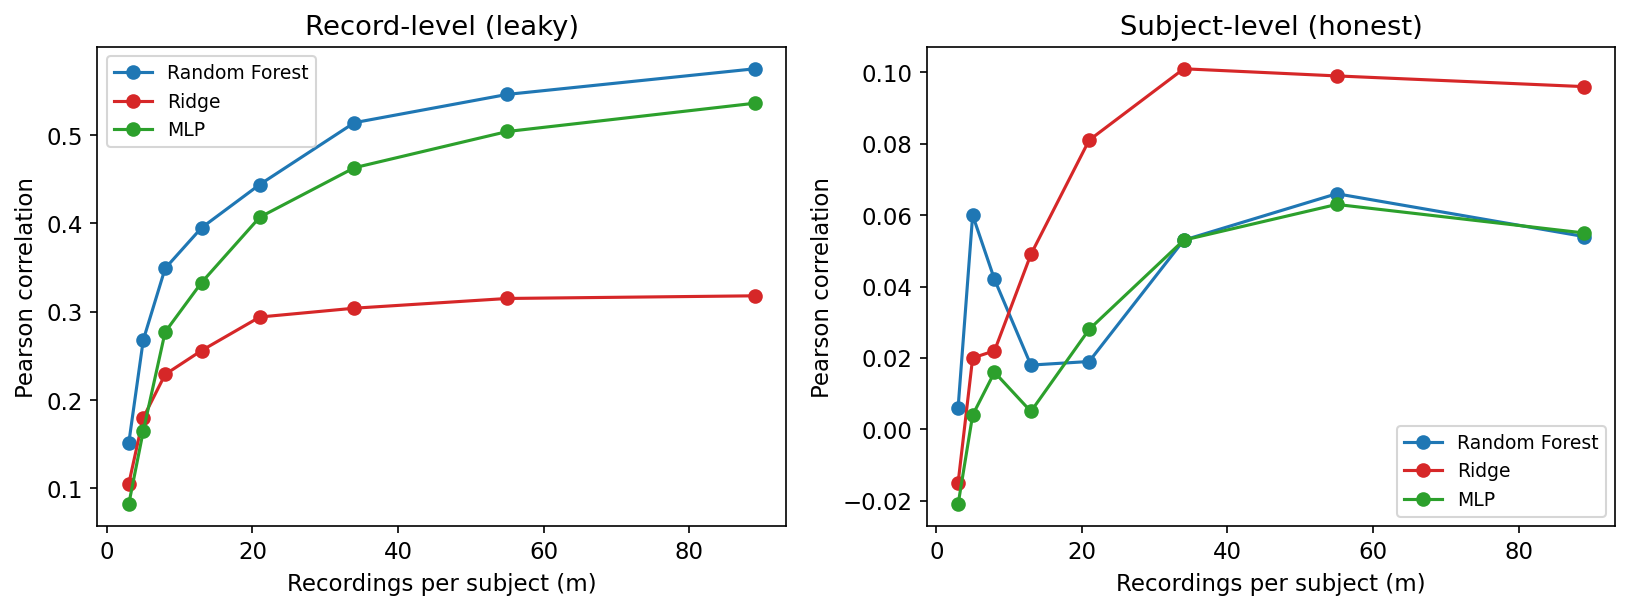
\includegraphics[width=\textwidth]{fig1.png}
\caption{Record-level (leaky, left) versus subject-level (honest, right) mean performance across the cluster-size sweep on the telemonitoring dataset (5 seeds). Leaky performance climbs steeply with cluster size for both the random forest and the MLP; honest performance stays flat and close to zero for every model, as expected if the climb on the left reflects growing opportunity to memorize subject identity rather than genuine generalization.}
\end{figure}

\subsection{Subject-level bootstrap confidence intervals confirm the gap is not a seed artifact}
Because the seed-level $t$-tests above hold the subject pool fixed, we additionally ran a subject-level cluster bootstrap for the random forest (Section 3.11, statistical-testing paragraph): resampling subjects with replacement, recomputing both protocols on each resample, and preserving each resampled subject's original identity as its group label so the honest protocol cannot be gamed by the resampling itself. We use 200 resamples for both Oxford and Sakar. The bootstrap gap estimates are: Oxford, mean gap $=0.196$ (95\% CI $[0.026, 0.407]$, gap $>0$ in 100\% of resamples); Sakar, mean gap $=0.130$ (95\% CI $[0.088, 0.183]$, gap $>0$ in 100\% of resamples). Figure 3 shows these intervals. Both bootstrap means land close to the seed-averaged point estimates in Table 2 (0.155 for Oxford random forest, 0.051 for Sakar random forest), and both confidence intervals exclude zero comfortably, giving an uncertainty-aware confirmation of the same effect reported in Table 2 rather than a materially different estimate of its size.

\begin{figure}[h]
\centering
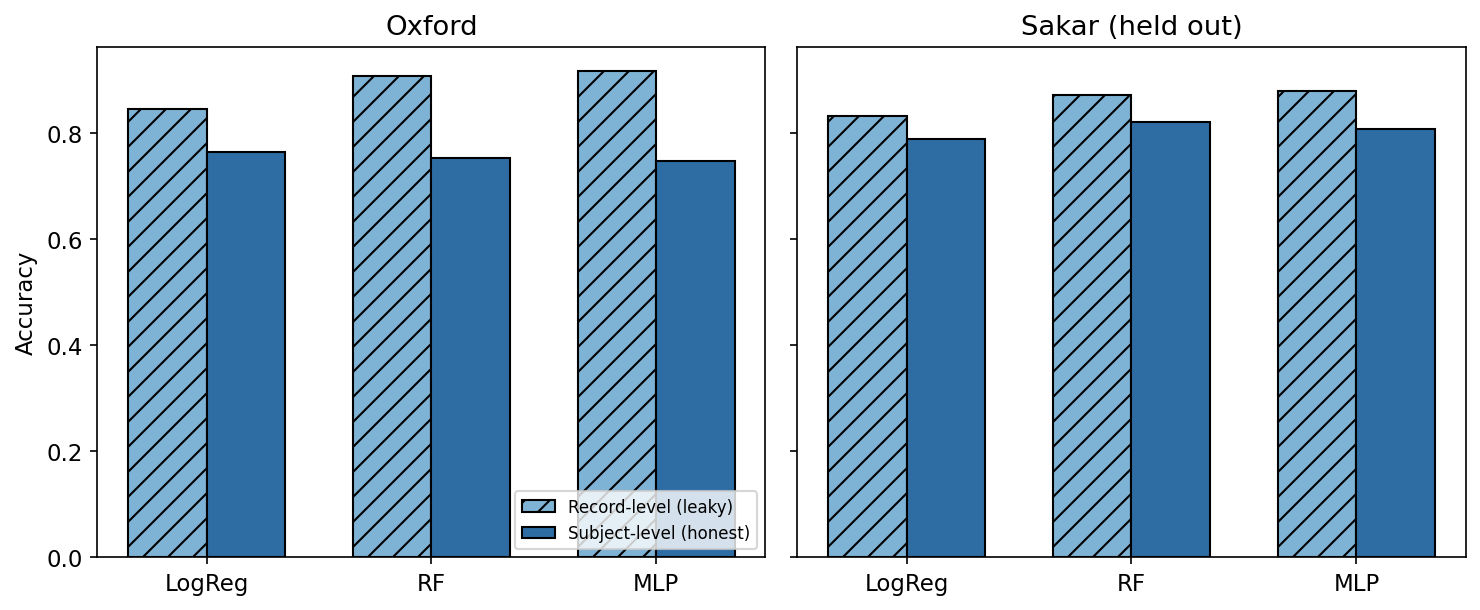
\includegraphics[width=0.85\textwidth]{fig2.png}
\caption{Record-level (hatched) versus subject-level (solid) accuracy on the two independent classification datasets, grouped by model so the leaky/honest pair for each model is visually adjacent. The gap is present for every model on both datasets and is larger on Oxford (larger design effect, Section 4.4) than on the held-out Sakar dataset.}
\end{figure}

\begin{figure}[h]
\centering
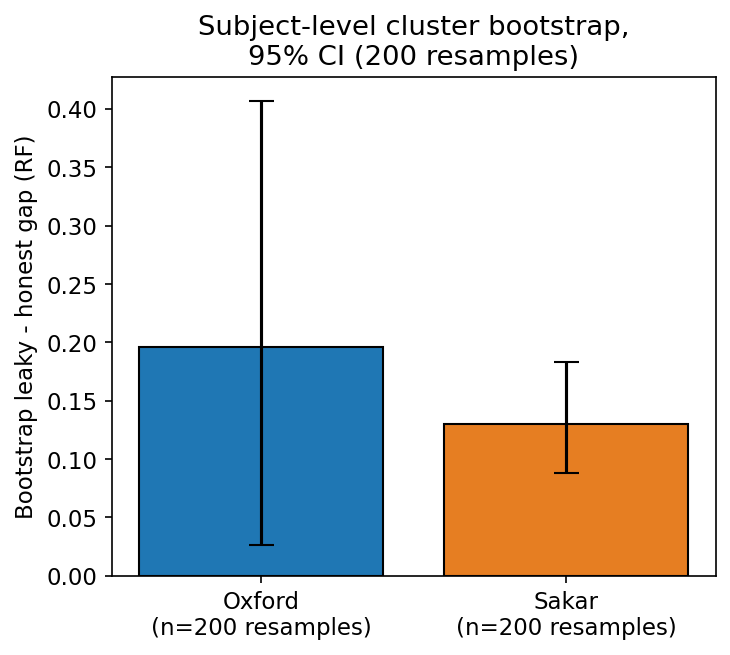
\includegraphics[width=0.7\textwidth]{fig3.png}
\caption{Subject-level cluster-bootstrap estimate of the leaky-honest gap (random forest), 200 resamples per dataset. Error bars show the 95\% percentile interval. The gap excludes zero comfortably in both datasets.}
\end{figure}

\subsection{The design effect tracks the size of the gap}
Figure 4 shows the measured gap from the telemonitoring sweep plotted against $\ln(\mathrm{DEFF})$, where $\mathrm{DEFF} = 1+(m-1)\cdot\mathrm{ICC}$ and ICC is estimated directly from the data (Section 3.6). A simple linear fit, $\mathrm{gap} \approx a\ln(\mathrm{DEFF})+b$, explains $R^2=0.906$ of the variance for the random forest ($p=2.7\times10^{-4}$), $R^2=0.572$ for ridge regression ($p=2.99\times10^{-2}$), and $R^2=0.919$ for the MLP ($p=2\times10^{-4}$), across the 8 points of the sweep for each model. We report these fits as evidence that $\ln(\mathrm{DEFF})$ is a useful, low-cost summary statistic for anticipating the scale of the leakage risk in a given dataset, not as a claim of a universal functional law; with only 8 points per model, the fitted $R^2$ should be read with that sample size in mind, which is why we treat the synthetic simulation (Section 4.6) as the stronger test of the underlying mechanism. Ridge regression's fit is noticeably weaker than the other two models' ($R^2=0.572$, still significant but with more scatter around the line); its gap curve is flatter and noisier overall (Table 1), which makes it harder for any two-parameter functional form to characterize precisely.

The identity also orders the two independent classification datasets in the same direction for all three models tested: Oxford has $\mathrm{DEFF} = 1+(6.09-1)\times0.744 = 4.79$; Sakar has $\mathrm{DEFF} = 1+(3-1)\times0.549 = 2.10$. Oxford's larger design effect is consistent with its larger gap for logistic regression (8.2 vs.\ 4.3 points), the random forest (15.5 vs.\ 5.1 points), and the MLP (16.9 vs.\ 7.1 points)---the identity orders all three models correctly in our data, not merely a majority of them. With only two datasets available for this check, we still treat it as a consistent but limited-sample observation rather than independent confirmation.

\begin{figure}[h]
\centering
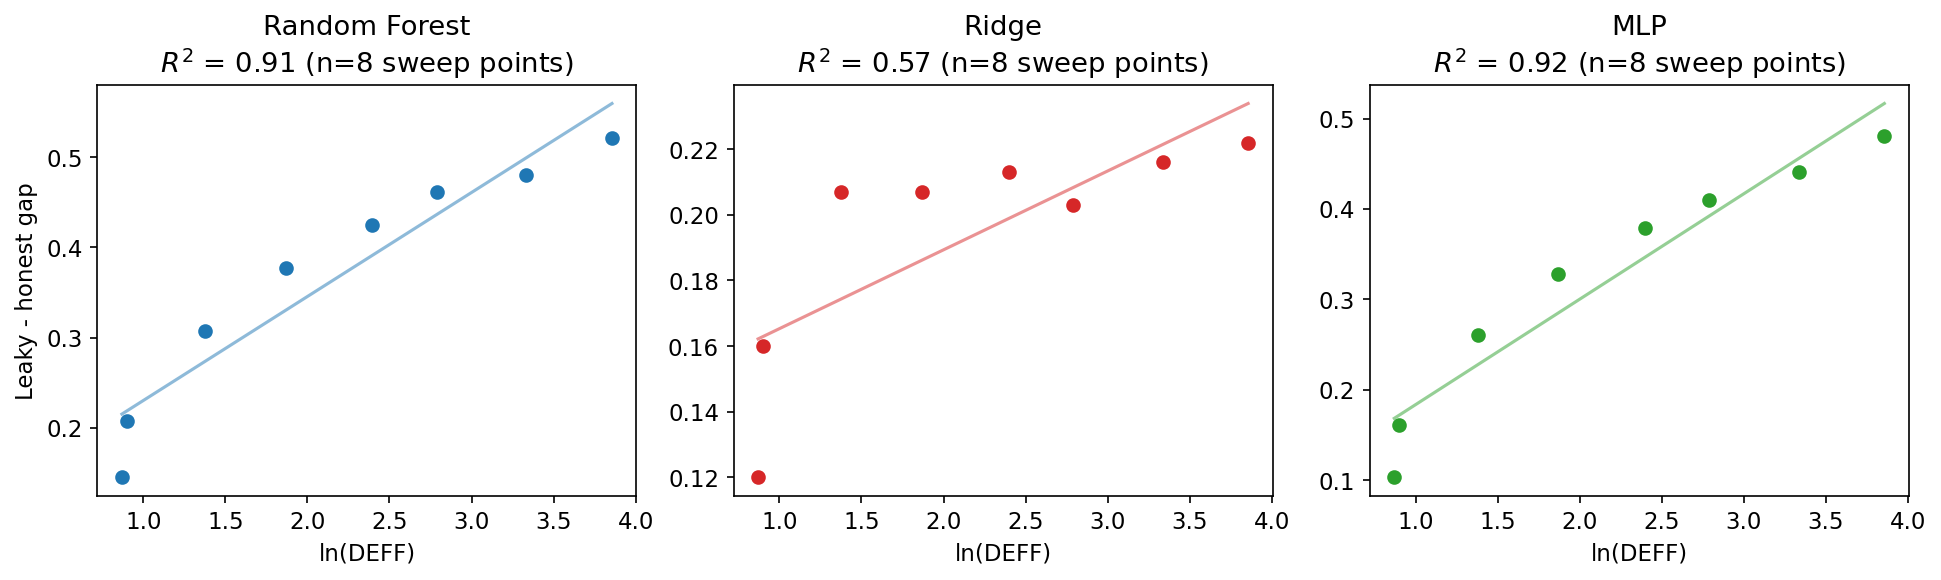
\includegraphics[width=\textwidth]{fig4.png}
\caption{Leaky-honest gap versus $\ln(\mathrm{DEFF})$ across the cluster-size sweep, with the fitted regression line per model. The classical survey-sampling design effect tracks 57--92\% of the variance in the measured leakage inflation across our 8 sweep points, depending on model; we treat this as suggestive given the small number of points, and validate the underlying mechanism independently in Figure 6.}
\end{figure}

\begin{table}[h]
\centering
\caption{Excess misdiagnoses per 1,000 newly screened patients if record-level accuracy is trusted as subject-level (real-world) accuracy.}
\begin{tabular}{llcc}
\toprule
Dataset & Model & Leaky acc.\ & Excess misdiagnoses / 1,000 \\
\midrule
Oxford & MLP & 91.7\% & 169 \\
Oxford & Random Forest & 90.8\% & 155 \\
Oxford & Logistic Reg.\ & 84.6\% & 82 \\
Sakar & MLP & 87.9\% & 71 \\
Sakar & Random Forest & 87.3\% & 51 \\
Sakar & Logistic Reg.\ & 83.3\% & 43 \\
\bottomrule
\end{tabular}
\end{table}

\subsection{A saturating-exponential mechanistic model fits the real sweep data better}
The log-linear DEFF fit above is a useful heuristic but does not, by itself, explain \textit{why} the gap should relate to $\ln(\mathrm{DEFF})$ in particular. Fitting the saturating-exponential model of Section 3.7 to the same sweep data gives, for the random forest, $G_{max}=0.482$, $\lambda=0.139$, $R^2=0.972$---a better fit than the log-linear DEFF model ($R^2=0.906$) with the same number of free parameters (Figure 5). The improvement holds for all three models, not only the random forest: ridge regression's saturating fit gives $G_{max}=0.213$, $\lambda=0.391$, $R^2=0.961$ (versus $R^2=0.572$ for the log-linear fit, its weakest showing of the three models above); the MLP's saturating fit gives $G_{max}=0.445$, $\lambda=0.114$, $R^2=0.978$, the best fit of any model, functional form, or dataset in this paper. That the saturating-exponential account outperforms the log-linear one across all three model families---including the linear model, where the mechanistic story of diminishing marginal memorization has the least obvious motivation---is, in our data, evidence that the functional form is picking up something more general about how the leaky-honest gap accumulates with cluster size than a story built specifically around high-capacity, non-linear models would predict.

\begin{figure}[h]
\centering
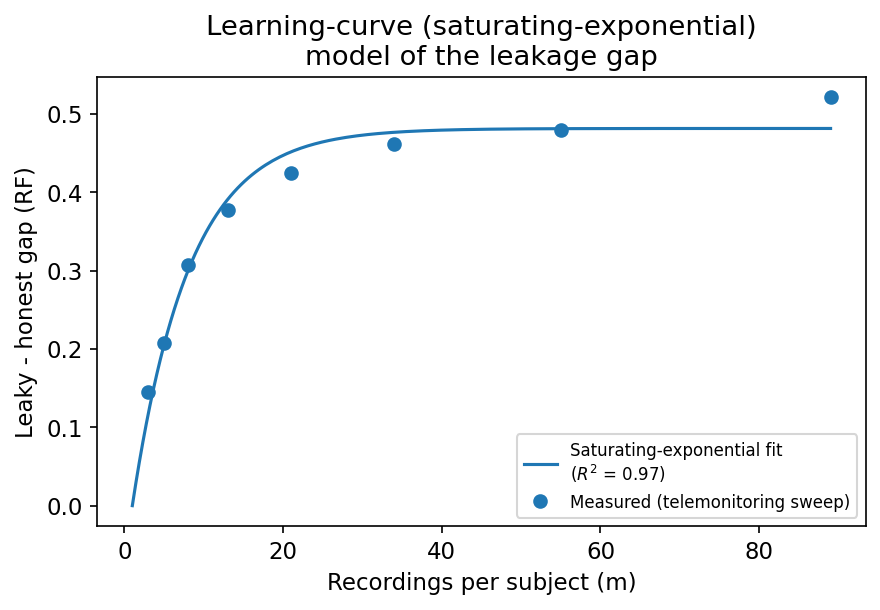
\includegraphics[width=0.7\textwidth]{fig5.png}
\caption{Saturating-exponential fit of the leaky-honest gap versus cluster size, random forest, telemonitoring sweep. This mechanistic account, motivated by diminishing marginal memorization opportunity per additional same-subject recording, fits the data better than the log-linear design-effect model.}
\end{figure}

\subsection{Independent synthetic simulation validates the ICC-scaling prediction}
Figure 6 shows results from the synthetic simulation described in Section 3.8, where cluster size and ICC are set directly (not estimated) and the true subject-level-generalizable accuracy is chance by construction. As predicted, the simulated leaky-honest gap is larger for higher ICC at every cluster size, and each ICC-conditional curve has the same saturating shape as the real sweep data (left panel). Fitting the saturating-exponential model separately at each of the 5 simulated ICC levels and regressing the fitted ceiling $G_{max}$ against ICC gives $R^2=0.987$ ($p=0.0006$) for the random forest and $R^2=0.998$ ($p<0.0001$) for logistic regression (right panel)---a linear ICC-to-ceiling relationship, exactly as the design-effect-motivated mechanism predicts, obtained on data where ICC and $m$ were experimentally assigned rather than estimated from an observational sample. Because the ground-truth label in this simulation is independent of the between-subject structure, any accuracy above 50\% under either protocol is attributable purely to clustering, which isolates the mechanism from any real, learnable Parkinson's-specific signal and is, in our view, the cleanest evidence in this paper that cluster size and intraclass correlation are jointly responsible for the leaky-honest gap, independent of the specific voice data or disease context.

\begin{figure}[h]
\centering
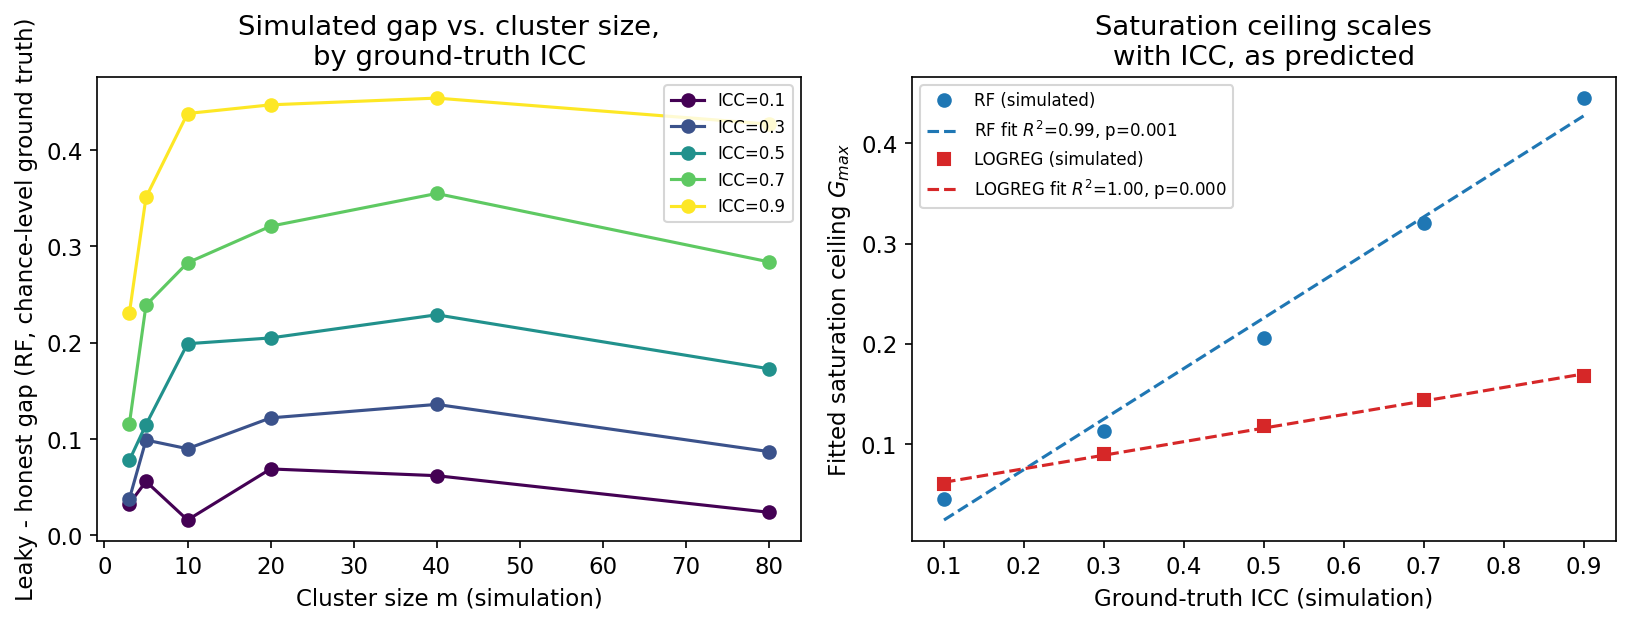
\includegraphics[width=\textwidth]{fig6.png}
\caption{Synthetic simulation with independently controlled ICC and cluster size $m$, ground-truth chance-level accuracy by construction. Left: simulated leaky-honest gap versus $m$, by ICC level, random forest. Right: the fitted saturation ceiling $G_{max}$ scales approximately linearly with ICC for both a random forest and logistic regression, matching the mechanism's prediction.}
\end{figure}

\subsection{The cost of trusting the wrong number}
Table 4 translates the measured gaps into excess misdiagnoses per 1,000 newly screened patients---the population a deployed tool would actually face, as opposed to the population of already-partially-seen subjects that record-level cross-validation implicitly evaluates on. The MLP on Oxford is the starkest case in our data: 169 excess misdiagnoses per 1,000 new patients relative to what the record-level number would lead a clinical team to expect, with the random forest close behind at 155. We keep this framing simple and accuracy-based (Section 3.9); Section 4.2 above already shows that this simplification specifically hides an asymmetry in \emph{which} error type drives the inflation, and it is intended to communicate the scale of the risk concretely, not as a substitute for a full clinical decision-cost analysis with asymmetric error costs in any specific deployment.

\subsection{Who benefits from the leak: a subject-level case study}
Figure 7 shows, for the Oxford dataset, each subject's leak advantage (their record-level minus subject-level per-recording accuracy under the random forest) against a separation ratio: their between-subject distinctiveness divided by their within-subject dispersion. The two are significantly correlated ($r=0.550$, $p=0.0011$, $n=32$). In our data, the subjects most responsible for the inflation are the ones with the most recognizable voices---exactly the subjects a memorization-capable classifier can most easily re-identify across recordings, independent of whether that voice belongs to a Parkinson's patient or a control.

\begin{figure}[h]
\centering
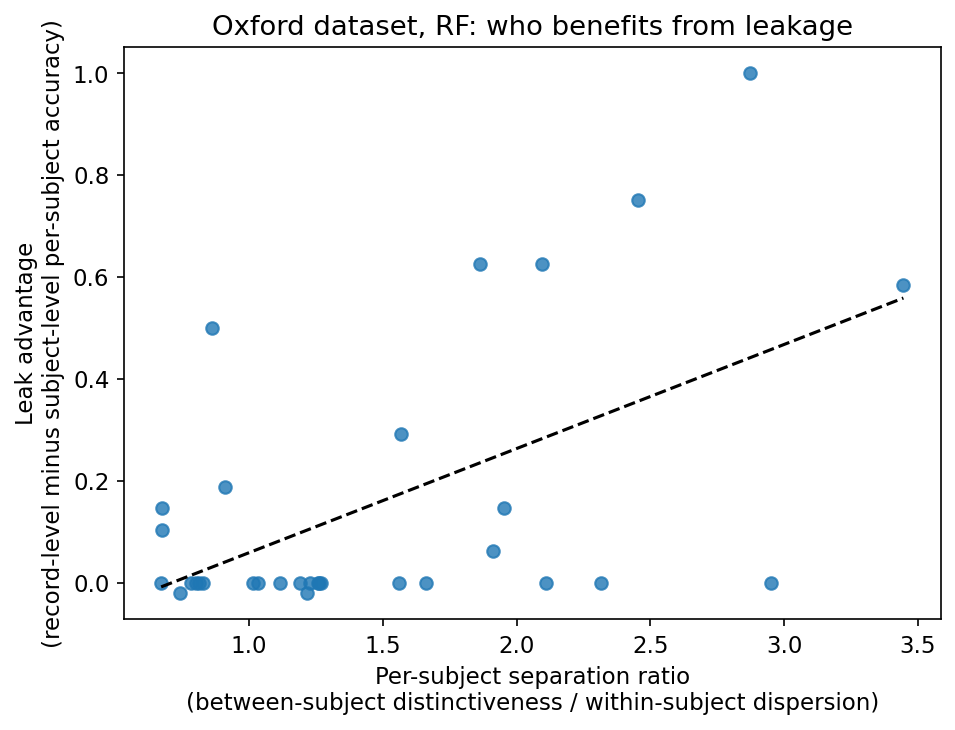
\includegraphics[width=0.7\textwidth]{fig7.png}
\caption{Per-subject leak advantage against the separation ratio (between-subject distinctiveness divided by within-subject dispersion), Oxford dataset, random forest. Subjects with the most distinctive voices contribute the most to the leaky protocol's inflated accuracy.}
\end{figure}

\section{Mechanism: why grouping fixes it}
\subsection{The design effect}
When $N$ measurements are drawn as $k$ clusters of $m$ correlated observations each rather than as $N$ independent observations, the effective information content of the sample is reduced. Kish's classical design effect \cite{kish1965} quantifies this:
\begin{equation}
\mathrm{DEFF} = 1 + (m-1)\cdot\mathrm{ICC},
\end{equation}
where ICC is the intraclass correlation, the fraction of total variance attributable to between-cluster (here, between-subject) differences. When $\mathrm{ICC}=0$ (recordings within a subject are no more similar to each other than to any other subject's recordings), $\mathrm{DEFF}=1$ and clustering is irrelevant. As ICC grows toward 1 (recordings within a subject are near-duplicates of each other), DEFF grows linearly in $m$: a dataset of $N=km$ recordings behaves, for the purpose of genuinely novel information, closer to a dataset of only $N/\mathrm{DEFF} \approx k$ independent points---the number of subjects, not the number of recordings.

Record-level cross-validation implicitly assumes $\mathrm{DEFF}=1$: it treats every recording as if it contributed independent information, when in fact, across our three voice datasets and the telemonitoring sweep, ICC is consistently substantial (roughly 0.37--0.74 depending on dataset and cluster size, Section 4.4), so much of what a flexible model appears to learn from additional recordings of an already-seen subject is not new information about Parkinson's disease. It is, to a substantial degree, the same subject, seen again.

\subsection{A saturating-exponential account}
The design-effect identity describes how much redundant, non-independent information is available in principle; it does not by itself specify the functional shape of how a model's exploitable advantage should grow with $m$. The saturating-exponential model of Section 3.7, $\mathrm{gap}(m) = G_{max}(1-e^{-\lambda(m-1)})$, adds a specific mechanistic hypothesis: a model's opportunity to memorize subject-specific structure has a capacity-limited ceiling $G_{max}$ (bounded by how much subject-identifying signal exists in the features and how much of it the model can represent), and each additional recording of an already-seen subject contributes a diminishing increment toward that ceiling. This fits the real telemonitoring sweep better than the log-linear DEFF fit for all three models tested (Section 4.5) and, in the independent simulation, correctly predicts that the fitted ceiling should scale linearly with ICC (Section 4.6)---a prediction we did not build into the simulation's data-generating process by construction, only into the model class we chose to fit to the simulation's output.

\subsection{Why capacity matters, and where a simple capacity story breaks down}
Both accounts describe the amount of redundant, non-independent information available to exploit; whether a given model actually exploits it depends on its capacity to represent subject-specific structure that has nothing to do with disease status. A linear model (ridge, logistic regression) can only exploit the redundancy to the extent that subject identity happens to align with a linear combination of the same features that carry disease signal, which is limited, and this is consistent with what we observe: the linear model shows the smallest, flattest gap of the three model families in every experiment in this paper (Tables 1--3). Where our data complicates a simple capacity story is in distinguishing between the two non-linear models: a naive prediction, that a random forest's greater representational flexibility should let it exploit subject-identity redundancy more thoroughly than an MLP, is not what we observe. Across the telemonitoring sweep, the two classification datasets, and the extended metrics in Table 3, the random forest and the MLP behave similarly to one another---sometimes the MLP shows the larger gap (Tables 2 and 3), sometimes the random forest does (Table 1 at most cluster sizes)---rather than one consistently dominating the other. We read this as evidence that capacity matters primarily as a linear-versus-nonlinear distinction in our data, separating models that can and cannot represent subject-specific structure at all, rather than as a fine-grained ranking that distinguishes between two different nonlinear model families. The synthetic simulation in Section 4.6, which only compares a random forest against logistic regression, does show the random forest reaching a higher $G_{max}$ than logistic regression at every simulated ICC level---consistent with the same linear-versus-nonlinear distinction, though it does not speak to the random-forest-versus-MLP comparison our real-data results raise.

\subsection{Why grouped cross-validation is the correct fix}
Subject-level (grouped) cross-validation removes the leak by construction: since no subject's recordings are ever split across the train/test boundary, a model cannot receive credit for recognizing a subject it has already seen, because it never sees a genuinely held-out recording from any subject it was trained on. This is a property of the evaluation partition, not of the model or the features. No post-hoc correction of the model's predictions can substitute for grouping the split correctly: the honest number can only be obtained by not leaking subject identity across the boundary in the first place. As Section 6 discusses, this fixes the identity-leakage channel specifically; it is not by itself a complete causal fix.

\section{Discussion}
\textbf{An old problem, examined with new quantitative tools.} That mixing repeated measurements from the same unit across train and test inflates apparent performance is not a new observation in statistics or in machine-learning-based science broadly \cite{kapoor2023}. Isolated reports within Parkinson's voice analysis \cite{omodunbi2025}, Alzheimer's MRI classification \cite{sifat2026}, inter-patient ECG classification \cite{dechazal2004}, connectome-based prediction \cite{rosenblatt2024}, and EEG sleep staging \cite{koksal2026} have flagged closely related failures. Our contribution is to move toward a more quantitative account within one domain: a controlled sweep showing the gap consistently increases with cluster size, a candidate closed-form identity and an independently motivated saturating-curve model that both relate to the size of the gap, replication across three independently collected datasets with one held out from all design decisions, subject-level bootstrap confidence intervals, an independent synthetic simulation, and a localization of which subjects drive the effect most in our case study.

\textbf{A causal-inference caveat: neither protocol is unbiased.} After circulating an earlier draft, Max A.\ Little (creator of the Oxford dataset) raised a point that we think deserves a dedicated discussion rather than a footnote, because it changes what we believe our central comparison actually shows. His argument, in the language of causal inference: subject identity, age, and gender are plausible confounders in this setting---common causes of both the acoustic features and the diagnostic label---and in the presence of such confounders, no purely statistical estimate based on features and labels alone, from either evaluation protocol, recovers the true causal relationship between voice and disease status \cite{pearl2009}. Record-level cross-validation is optimistically biased because identity leaks directly across the split, which is the failure mode this paper quantifies. But subject-level cross-validation is not thereby an unbiased estimate of population-level generalization either: holding out entire subjects means the training and test partitions no longer share a single distribution, since each subject carries their own idiosyncratic shift, and classical cross-validation's validity depends on train and test being drawn from the same distribution. Subject-level splitting satisfies that assumption no better than record-level splitting does---it fails it in the opposite direction, trading a positive (optimistic) bias for a negative one induced by domain and label shift across held-out individuals.

Little and Badawy's causal bootstrapping framework \cite{little2019} offers a partial remedy: for confounders like age or gender, one can use back-door adjustment (stratification, or resampling schemes that simulate an interventional distribution from observational data) to obtain a causally meaningful estimate without this trade-off. Subject identity, however, is a harder case, because it is a deterministic, one-value-per-individual confounder: every recording has exactly one true subject, so there is no repeated variation in identity within a subject to adjust over, which leaves a structural gap in the joint distribution that back-door adjustment cannot fill from the data as collected. Little describes closing this gap for identity confounding specifically as an open research problem.

Given this, we want to be precise about what our results do and do not show. The leaky-honest gap we measure throughout this paper is real, reproducible across three independent datasets, related in a consistent way to cluster size and intraclass correlation, and validated with an independent simulation and subject-level bootstrap---but it should be read as a measurement of the size of the identity-leakage channel that record-level cross-validation opens, not as a measurement of the distance between a biased estimate and the one true population-level accuracy. The subject-level number we call ``honest'' throughout is better understood as a different, differently biased estimate that happens to close the specific leak we set out to study, rather than as ground truth. We think this sharpens, rather than undermines, our practical recommendation below: grouped cross-validation is still the right way to remove subject-identity leakage specifically, but neither number should be reported or interpreted as an unbiased estimate of real-world diagnostic accuracy without further causal adjustment, and we now say so explicitly rather than only in this limitations-adjacent discussion.

\textbf{Practical recommendation.} Based on our results, we suggest that datasets in neurodegenerative-disease machine learning built from repeated per-subject measurements---voice recordings, gait trials, repeated cognitive tests, longitudinal imaging---be evaluated with subject- or patient-grouped cross-validation by default, and that record-level numbers, where reported at all, be clearly labeled as an upper bound on performance rather than an estimate of it. We suggest turning the design effect from a post-hoc explanatory tool into a pre-registration-style checklist item: before running any evaluation, a researcher can compute $m$ (mean recordings per subject) and the intraclass correlation of the feature set, plug both into $\mathrm{DEFF} = 1+(m-1)\cdot\mathrm{ICC}$, and treat the resulting value as an inexpensive, five-minute diagnostic. In our data, every dataset with $\mathrm{DEFF} > 1.5$ showed a record-level inflation large enough to change a model's apparent performance tier (Oxford's $\mathrm{DEFF}=4.79$ corresponded to gaps of 8.2--16.9 points depending on model; Sakar's $\mathrm{DEFF}=2.10$ still corresponded to gaps of 4.3--7.1 points); we do not have enough datasets to calibrate this threshold precisely, but we suggest $\mathrm{DEFF} > 1.5$ as a provisional red flag that record-level cross-validation on a given dataset should not be trusted without a grouped re-analysis, and that reporting DEFF alongside any accuracy number, using Eq.\ (1), costs a reviewer nothing to check and a reader nothing to interpret.

\textbf{What is and is not new here.} Grouped cross-validation itself is standard practice where it is used, and the design effect is decades-old survey-sampling theory \cite{kish1965}; we invent neither. What we add is an attempt to connect these off-the-shelf ideas to a quantitative, testable account of the size of the inflation a given dataset and model combination will show, supported across a controlled real-data sweep, an independent ground-truth-controlled simulation, and bootstrap-based uncertainty quantification---while being explicit that our evidence comes from a small number of real datasets in one modality (voice), and that the identity should be treated as a useful heuristic rather than an established universal law until tested more broadly.

\textbf{Beyond Parkinson's voice analysis.} The design-effect and saturating-curve accounts in Eq.\ (1) and Section 5 are not written in terms of anything specific to voice or to Parkinson's disease, and the qualitative failure mode---clustered, repeated measurements per patient, evaluated without uniformly adopting grouped cross-validation---has been separately reported in Alzheimer's disease neuroimaging \cite{sifat2026}, ECG \cite{dechazal2004}, functional connectomics \cite{rosenblatt2024}, and EEG sleep staging \cite{koksal2026}. We hypothesize, but have not directly tested, that the same quantitative relationship would hold in these other repeated-measures settings; confirming that is a natural direction for future work rather than a claim we make here.

\textbf{Limitations.} The most important limitation is the causal one discussed in Section 6: our results characterize the size of the identity-leakage bias in record-level cross-validation relative to subject-level cross-validation, not an unbiased estimate of true population-level generalization, which neither protocol provides in the presence of subject-identity, age, and gender confounding. We study voice-based assessment specifically and three datasets, all secondary/derived tabular feature sets rather than raw audio; whether the same relationships hold for models trained end-to-end on raw waveforms or spectrograms is untested here. A more basic limitation than either of those is that our entire cluster-size sweep---the core evidence for the claim that the leaky-honest gap scales in a predictable way with $m$---comes from a single dataset (telemonitoring) in a single modality (voice), because it is the only one of the three with enough recordings per subject to support a wide sweep. Everything in Sections 4.1, 4.4, and 4.5 that describes how the gap grows with $m$ is therefore, strictly speaking, a within-dataset finding; the design-effect fits in Section 4.4 rest on 8 sweep points per model, and the cross-dataset ordering check rests on only two datasets, so both should be read as consistent with, rather than independent statistical confirmation of, the identity. Whether the same $m$-scaling curve would hold on a different voice-recording protocol, let alone a different modality (gait, imaging, ECG), is untested here and is the single biggest open question the synthetic simulation in Section 4.6 was designed to partially address, since it at least confirms the mechanism does not depend on anything specific to this one dataset's acoustic features. The synthetic simulation (Section 4.6) substantially strengthens the mechanistic case by removing dependence on any single real dataset, but it necessarily simplifies the data-generating process (linear, additive, Gaussian subject and noise effects) relative to real acoustic features, and the ICC-versus-$m$ grid we sweep is not exhaustive, only sufficient to establish the predicted linear ICC-to-ceiling relationship at the 5 levels we test. Our subject-level bootstrap (Section 4.3) is restricted to the random forest, for compute-budget reasons, at 200 resamples per dataset; extending it to all three models, and to more resamples, would further strengthen the evidence, though 200 resamples with a 95\% CI that excludes zero comfortably in both datasets is a reasonably well-powered estimate for the qualitative claim we make. The finding that we believe deserves the most caution going forward is the departure from a simple capacity-based ordering documented in Sections 4.1--4.3 and revisited in Section 5.3: our data show the random forest and MLP behaving similarly to one another rather than one uniformly dominating the other, which is a real pattern in our results but one we observed rather than predicted in advance, and it should be treated as an empirical finding specific to these three datasets and this feature representation rather than a general claim about model capacity and leakage. Our consequence framing (Sections 3.9, 4.7) uses accuracy directly rather than a full clinical cost model with asymmetric error costs; Section 4.2 partially addresses this by showing the honest-protocol accuracy drop is driven predominantly by false positives rather than false negatives across every model and dataset, but a deployment-ready estimate would still need the leaky-versus-honest gap weighted by whatever cost ratio a given clinical context assigns to the two error types, which we did not do here. The qualitative conclusion, that record-level numbers overstate real-world performance by a clinically non-trivial margin in our data, does not depend on that simplification, but the exact magnitude, and which error type drives it in a specific deployment, would.

\section{Conclusion}
Voice-based Parkinson's disease datasets are, by design, built from several recordings per subject, and the most common way of evaluating models on them---randomly splitting recordings into folds---lets that repeated structure leak subject identity across the evaluation boundary. We measured this leak directly across three independent datasets: it inflates reported accuracy by up to 16.9 points on a real classification dataset and produces a correlation gap that consistently increases from 0.14 to 0.52 as more recordings per subject become available to memorize, for a random forest, with a comparably large effect for an MLP; a linear model shows a smaller, flatter version of the same effect. A classical survey-sampling identity, the design effect, tracks the size of this gap with $R^2$ up to 0.92 via a log-linear fit and up to 0.98 via a saturating-exponential fit across our sweep, a finding we support with an independent synthetic simulation confirming the predicted ICC-scaling of that model's ceiling, and subject-level bootstrap confidence intervals (200 resamples per dataset) that keep the gap above zero in every resample we ran. The inflation is not symmetric across error types: in every model and dataset we test, it is driven predominantly by a rise in false-positive rate rather than false-negative rate. Trusting the leaky number, rather than the honest one, corresponds in our data to dozens to well over a hundred excess misdiagnoses per 1,000 new patients, depending on model and dataset. Grouping cross-validation folds by subject removes this specific leak by construction; our results suggest it should be treated as the default reporting standard for this literature rather than an optional robustness check. As a concrete, low-cost first step, we suggest computing $\mathrm{DEFF}=1+(m-1)\cdot\mathrm{ICC}$ for any repeated-measures dataset before trusting a record-level number at all; in our data a $\mathrm{DEFF}$ above roughly 1.5 flagged every case where the leakage-driven inflation was large enough to matter. We are explicit, however, that this grouped number is not itself an unbiased estimate of population-level generalization (Section 6): it closes the identity-leakage channel we studied, but subject identity, age, and gender remain confounders that classical cross-validation of either kind cannot fully adjust for, and closing that remaining gap is, as far as we are aware, an open problem.

\section*{Data and Code Availability}
All three datasets are public: the Oxford Parkinson's voice dataset \cite{little2007} and the Sakar et al.\ speech dataset \cite{sakar2019} are distributed via the UCI Machine Learning Repository; the Tsanas et al.\ telemonitoring dataset \cite{tsanas2010} is likewise public via UCI. All experiment code (data loading, cluster-size subsampling, both cross-validation protocols, the ICC/design-effect computation, the saturating-exponential fits, the synthetic simulation, the subject-level bootstrap, the consequence framing, the case-study analysis, and figure generation), with fixed random seeds, is available at \url{https://github.com/Muhammadjon-crypto/PD-Voice-Leakage-Audit}.

\section*{Author Contributions}
Mustafojon Tursunbadalov and Muhammadjon Tursunbadalov contributed equally to this work. Both authors jointly designed the study, implemented the experiments, analyzed the results, and wrote the manuscript. Bekir Karlik reviewed an earlier draft and proposed the methodological revisions incorporated in this version, including expanding the subject-level bootstrap to 200 resamples per dataset, reporting F1, MCC, and the false-negative/false-positive error-rate breakdown alongside accuracy, and framing the design effect as a pre-analysis diagnostic threshold; he provided guidance on the resulting revisions but did not implement the experiments himself.

\section*{Conflicts of Interest}
The authors declare no competing interests.

\begin{thebibliography}{99}
\bibitem{kapoor2023} Kapoor, S.; Narayanan, A. Leakage and the Reproducibility Crisis in Machine-Learning-Based Science. \textit{Patterns} \textbf{2023}, \textit{4}, 100804.
\bibitem{little2007} Little, M. A.; McSharry, P. E.; Roberts, S. J.; Costello, D. A. E.; Moroz, I. M. Exploiting Nonlinear Recurrence and Fractal Scaling Properties for Voice Disorder Detection. \textit{BioMedical Engineering OnLine} \textbf{2007}, \textit{6}, 23.
\bibitem{sakar2019} Sakar, C. O.; Serbes, G.; Gunduz, A.; Tunc, H. C.; Nizam, H.; Sakar, B. E.; Tutuncu, M.; Aydin, T.; Isenkul, M. E.; Apaydin, H. A Comparative Analysis of Speech Signal Processing Algorithms for Parkinson's Disease Classification and the Use of the Tunable Q-Factor Wavelet Transform. \textit{Applied Soft Computing} \textbf{2019}, \textit{74}, 255--263.
\bibitem{tsanas2010} Tsanas, A.; Little, M. A.; McSharry, P. E.; Ramig, L. O. Accurate Telemonitoring of Parkinson's Disease Progression by Noninvasive Speech Tests. \textit{IEEE Transactions on Biomedical Engineering} \textbf{2010}, \textit{57}, 884--893.
\bibitem{omodunbi2025} Omodunbi, B. A.; Olawade, D. B.; Awe, O. F.; Soladoye, A. A.; Aderinto, N.; Ovsepian, S. V.; Boussios, S. Stacked Ensemble Learning for Classification of Parkinson's Disease Using Telemonitoring Vocal Features. \textit{Diagnostics} \textbf{2025}, \textit{15}, 1467.
\bibitem{sifat2026} Sifat, M.; Akter, S.; Islam, A.; et al. 3D MRI-Based Alzheimer's Disease Classification Using Multi-Modal 3D CNN with Leakage-Aware Subject-Level Evaluation. \textit{arXiv:2603.17304}, 2026.
\bibitem{dechazal2004} de Chazal, P.; O'Dwyer, M.; Reilly, R. B. Automatic Classification of Heartbeats Using ECG Morphology and Heartbeat Interval Features. \textit{IEEE Transactions on Biomedical Engineering} \textbf{2004}, \textit{51}, 1196--1206.
\bibitem{rosenblatt2024} Rosenblatt, M.; Tejavibulya, L.; Jiang, R.; Noble, S.; Scheinost, D. Data Leakage Inflates Prediction Performance in Connectome-Based Machine Learning Models. \textit{Nature Communications} \textbf{2024}, \textit{15}, 1829.
\bibitem{koksal2026} K{\"o}ksal, A. S. Cross-Validation and Normalization in EEG Sleep Staging: Impacts on Generalization, Calibration, and Clinical Validity. \textit{D{\"u}zce University Journal of Science and Technology} \textbf{2026}, \textit{14}, 72--85.
\bibitem{little2019} Little, M. A.; Badawy, R. Causal Bootstrapping. \textit{arXiv:1910.09648}, 2019.
\bibitem{pearl2009} Pearl, J. \textit{Causality: Models, Reasoning, and Inference}, 2nd ed.; Cambridge University Press: Cambridge, 2009.
\bibitem{kish1965} Kish, L. \textit{Survey Sampling}; John Wiley \& Sons: New York, 1965.
\bibitem{shrout1979} Shrout, P. E.; Fleiss, J. L. Intraclass Correlations: Uses in Assessing Rater Reliability. \textit{Psychological Bulletin} \textbf{1979}, \textit{86}, 420--428.
\bibitem{pedregosa2011} Pedregosa, F.; Varoquaux, G.; Gramfort, A.; Michel, V.; Thirion, B.; Grisel, O.; Blondel, M.; Prettenhofer, P.; Weiss, R.; Dubourg, V.; Vanderplas, J.; Passos, A.; Cournapeau, D.; Brucher, M.; Perrot, M.; Duchesnay, E. Scikit-learn: Machine Learning in Python. \textit{Journal of Machine Learning Research} \textbf{2011}, \textit{12}, 2825--2830.
\bibitem{hunter2007} Hunter, J. D. Matplotlib: A 2D Graphics Environment. \textit{Computing in Science \& Engineering} \textbf{2007}, \textit{9}, 90--95.
\end{thebibliography}

\end{document}
